\documentclass[12pt]{amsart}

% PACKAGES
\usepackage{amsmath}
\usepackage{amssymb}
\usepackage{amsfonts}
\usepackage[alphabetic]{amsrefs}
\usepackage{amsthm}
% \usepackage{enumitem}
\usepackage{enumerate}
\usepackage{fullpage}
\usepackage{color}
\usepackage{graphicx}
\usepackage{wrapfig}
\usepackage{hyperref}
\usepackage{microtype}
\usepackage{tikz}
\usepackage{float}
\usepackage{caption}
\usepackage{quiver}
%\hypersetup{linktoc = all, colorlinks = true, urlcolor = Blue, linkcolor = Red, citecolor = RoyalBlue}
\usepackage[parfill]{parskip}

% COMMANDS 
\newcommand{\nc}{\newcommand}
\newcommand{\rc}{\renewcommand}
\nc{\on}{\operatorname}

% EDITING
\definecolor{red}{rgb}{1,0,0}
\definecolor{orange}{rgb}{1,0.5,0}
\definecolor{purple}{rgb}{.5,.2,.8}
\definecolor{blue}{rgb}{.2,.2,.8}
\definecolor{green}{rgb}{.4,.6,.4}
\newcommand{\question}[1]{\noindent  \textcolor{red}{Question: #1}}
\newcommand{\todo}[1]{\noindent  \textcolor{blue}{To do: #1}}
% Editing line spacing
% \linespread{1.5}

% BLACKBOARD BOLD
\rc{\AA}{\mathbb{A}}	
\nc{\BB}{\mathbb{B}}	
\nc{\CC}{\mathbb{C}}	
\nc{\DD}{\mathbb{D}}	
\nc{\EE}{\mathbb{E}}	
\nc{\FF}{\mathbb{F}}	
\nc{\GG}{\mathbb{G}}	
\nc{\HH}{\mathbb{H}}	
\nc{\II}{\mathbb{I}}	
\nc{\JJ}{\mathbb{J}}	
\nc{\KK}{\mathbb{K}}	
\nc{\LL}{\mathbb{L}}	
\nc{\MM}{\mathbb{M}}	
\nc{\NN}{\mathbb{N}}	
\nc{\OO}{\mathbb{O}}	
\nc{\PP}{\mathbb{P}}	
\nc{\QQ}{\mathbb{Q}}	
\nc{\RR}{\mathbb{R}}	
\rc{\SS}{\mathbb{S}}	
\nc{\TT}{\mathbb{T}}	
\nc{\UU}{\mathbb{U}}	
\nc{\VV}{\mathbb{V}}	
\nc{\WW}{\mathbb{W}}	
\nc{\XX}{\mathbb{X}}	
\nc{\YY}{\mathbb{Y}}	
\nc{\ZZ}{\mathbb{Z}}	

% BOLD FACE
\nc{\bA}{\mathbf{A}}	
\nc{\bB}{\mathbf{B}}	
\nc{\bC}{\mathbf{C}}	
\nc{\bD}{\mathbf{D}}	
\nc{\bE}{\mathbf{E}}	
\nc{\bF}{\mathbf{F}}	
\nc{\bG}{\mathbf{G}}	
\nc{\bH}{\mathbf{H}}	
\nc{\bI}{\mathbf{I}}	
\nc{\bJ}{\mathbf{J}}	
\nc{\bK}{\mathbf{K}}	
\nc{\bL}{\mathbf{L}}	
\nc{\bM}{\mathbf{M}}	
\nc{\bN}{\mathbf{N}}	
\nc{\bO}{\mathbf{O}}	
\nc{\bP}{\mathbf{P}}	
\nc{\bQ}{\mathbf{Q}}	
\nc{\bR}{\mathbf{R}}	
\nc{\bS}{\mathbf{S}}	
\nc{\bT}{\mathbf{T}}	
\nc{\bU}{\mathbf{U}}	
\nc{\bV}{\mathbf{V}}	
\nc{\bW}{\mathbf{W}}	
\nc{\bX}{\mathbf{X}}	
\nc{\bY}{\mathbf{Y}}	
\nc{\bZ}{\mathbf{Z}}	

% CALLIGRAPHIC
\nc{\calA}{\mathcal{A}}	
\nc{\calB}{\mathcal{B}}	
\nc{\calC}{\mathcal{C}}	
\nc{\calD}{\mathcal{D}}	
\nc{\calE}{\mathcal{E}}	
\nc{\calF}{\mathcal{F}}	
\nc{\calG}{\mathcal{G}}	
\nc{\calH}{\mathcal{H}}	
\nc{\calI}{\mathcal{I}}	
\nc{\calJ}{\mathcal{J}}	
\nc{\calK}{\mathcal{K}}	
\nc{\calL}{\mathcal{L}}	
\nc{\calM}{\mathcal{M}}	
\nc{\calN}{\mathcal{N}}	
\nc{\calO}{\mathcal{O}}	
\nc{\calP}{\mathcal{P}}	
\nc{\calQ}{\mathcal{Q}}	
\nc{\calR}{\mathcal{R}}	
\nc{\calS}{\mathcal{S}}
\nc{\calT}{\mathcal{T}}	
\nc{\calU}{\mathcal{U}}	
\nc{\calV}{\mathcal{V}}	
\nc{\calW}{\mathcal{W}}
\nc{\calX}{\mathcal{X}}	
\nc{\calY}{\mathcal{Y}}	
\nc{\calZ}{\mathcal{Z}}

% LOWERCASE FRAK
\nc{\fraka}{\mathfrak{a}}
\nc{\frakb}{\mathfrak{b}}
\nc{\frakc}{\mathfrak{c}}
\nc{\frakd}{\mathfrak{d}}
\nc{\frake}{\mathfrak{e}}
\nc{\frakf}{\mathfrak{f}}
\nc{\frakg}{\mathfrak{g}}
\nc{\frakh}{\mathfrak{h}}
\nc{\fraki}{\mathfrak{i}}
\nc{\frakj}{\mathfrak{j}}
\nc{\frakk}{\mathfrak{k}}
\nc{\frakl}{\mathfrak{l}}
\nc{\frakm}{\mathfrak{m}}
\nc{\frakn}{\mathfrak{n}}
\nc{\frako}{\mathfrak{o}}
\nc{\frakp}{\mathfrak{p}}
\nc{\frakq}{\mathfrak{q}}
\nc{\frakr}{\mathfrak{r}}
\nc{\fraks}{\mathfrak{s}}
\nc{\frakt}{\mathfrak{t}}
\nc{\fraku}{\mathfrak{u}}
\nc{\frakv}{\mathfrak{v}}
\nc{\frakw}{\mathfrak{w}}
\nc{\frakx}{\mathfrak{x}}
\nc{\fraky}{\mathfrak{y}}
\nc{\frakz}{\mathfrak{z}}

% UPPERCASE FRAK
\nc{\frakA}{\mathfrak{A}}
\nc{\frakB}{\mathfrak{B}}
\nc{\frakC}{\mathfrak{C}}
\nc{\frakD}{\mathfrak{D}}
\nc{\frakE}{\mathfrak{E}}
\nc{\frakF}{\mathfrak{F}}
\nc{\frakG}{\mathfrak{G}}
\nc{\frakH}{\mathfrak{H}}
\nc{\frakI}{\mathfrak{I}}
\nc{\frakJ}{\mathfrak{J}}
\nc{\frakK}{\mathfrak{K}}
\nc{\frakL}{\mathfrak{L}}
\nc{\frakM}{\mathfrak{M}}
\nc{\frakN}{\mathfrak{N}}
\nc{\frakO}{\mathfrak{O}}
\nc{\frakP}{\mathfrak{P}}
\nc{\frakQ}{\mathfrak{Q}}
\nc{\frakR}{\mathfrak{R}}
\nc{\frakS}{\mathfrak{S}}
\nc{\frakT}{\mathfrak{T}}
\nc{\frakU}{\mathfrak{U}}
\nc{\frakV}{\mathfrak{V}}
\nc{\frakW}{\mathfrak{W}}
\nc{\frakX}{\mathfrak{X}}
\nc{\frakY}{\mathfrak{Y}}
\nc{\frakZ}{\mathfrak{Z}}

% OPERATORS
\nc{\Lie}{\on{Lie}}
\nc{\GL}{\on{GL}}
\nc{\PGL}{\on{PGL}}
\nc{\SL}{\on{SL}}
\nc{\Sp}{\on{Sp}}
\nc{\GSp}{\on{GSp}}
\nc{\SO}{\on{SO}}
\nc{\Or}{\on{O}}
\nc{\gl}{\on{\mathfrak{gl}}}
\rc{\sl}{\on{\mathfrak{sl}}}
\nc{\git}{/\!\!/}

\nc{\Mat}{\on{Mat}}
\nc{\Fun}{\on{Fun}}
\nc{\Aut}{\on{Aut}}
\nc{\End}{\on{End}}
\nc{\Hom}{\on{Hom}}
\nc{\Sym}{\on{Sym}}
\nc{\Span}{\on{span}}
\nc{\Irr}{\on{Irr}}
\nc{\Uch}{\on{Uch}}
\nc{\Type}{\on{Type}}
\nc{\Spec}{\on{Spec}}

\nc{\Ind}{\on{Ind}}
\nc{\Res}{\on{Res}}
\nc{\stab}{\on{stab}}
\nc{\orb}{\on{orb}}
\rc{\ker}{\on{ker}}
\nc{\im}{\on{im}}
\nc{\tr}{\on{tr}}
\nc{\ord}{\on{ord}}
\nc{\Tor}{\on{Tor}}
\nc{\Ad}{\on{Ad}}

\nc{\Id}{\on{Id}}
\nc{\Log}{\on{Log}}
\nc{\Exp}{\on{Exp}}
\nc{\Frac}{\on{Frac}}
\nc{\diag}{\on{diag}}
\nc{\D}{\on{D}}

% MATHRM
\nc{\St}{\mathrm{St}}
\nc{\triv}{\mathrm{triv}}
\nc{\sgn}{\mathrm{sgn}}
\nc{\reg}{\mathrm{reg}}
\nc{\rank}{\mathrm{rank}}
\nc{\op}{\mathrm{op}}
\nc{\ad}{\mathrm{ad}}
\rc{\ss}{\mathrm{ss}}
\nc{\HLV}{\mathrm{HLV}}

% ENVIRONMENTS
\theoremstyle{plain}
\newtheorem{theorem}{Theorem}%[subsection]
\newtheorem{definition}[theorem]{Definition}
\newtheorem{corollary}[theorem]{Corollary}
\newtheorem{lemma}[theorem]{Lemma}
\newtheorem{proposition}[theorem]{Proposition}
\newtheorem{claim}[theorem]{Claim}
\newtheorem{example}[theorem]{Example}
\newtheorem{remark}[theorem]{Remark}

% CONE PLOTTING
\usepackage{graphicx} % For including graphics
\usepackage{subcaption} % For subfigures
\usepackage{tikz}
\usepackage{amsmath}
\usepackage{pgfplots}
\pgfplotsset{compat=1.17}
\usepackage{tikz,tikz-3dplot}
\tdplotsetmaincoords{80}{45}
\tdplotsetrotatedcoords{-90}{180}{-90}

%% style for surfaces
\tikzset{surface/.style={draw=gray!70!black, fill=gray!40!white, fill opacity=.6}}

%% macros to draw back and front of cones
%% optional first argument is styling; others are z, radius, side offset (in degrees)
\newcommand{\coneback}[4][]{
  %% start at the correct point on the circle, draw the arc, then draw to the origin of the diagram, then close the path
  \draw[canvas is xy plane at z=#2, #1] (45-#4:#3) arc (45-#4:225+#4:#3) -- (O) --cycle;
}
\newcommand{\conefront}[4][]{
  \draw[canvas is xy plane at z=#2, #1] (45-#4:#3) arc (45-#4:-135+#4:#3) -- (O) --cycle;
}

\allowdisplaybreaks

\begin{document}
\pagenumbering{roman}

%%%%%%%%%%%%%%%%%%%%%%%%%%%%%%%%%%%%%%%%%%%%%%%%%%%%%%%%%%%%%%%%%%%%%%%%%%%%%%%%
% Title Page
%%%%%%%%%%%%%%%%%%%%%%%%%%%%%%%%%%%%%%%%%%%%%%%%%%%%%%%%%%%%%%%%%%%%%%%%%%%%%%%%
\begin{center}
\includegraphics[width=10cm]{../images/UQLogo.jpg} \\ 
\vspace{3cm}
{\LARGE\textsc{Mid-year Review}} \\
{\textsc{July 2024}} \\
\vspace{0.5cm}
{\textsc{Declan Fletcher}} \\
\vspace{5cm}
{\textsc{Supervisor: \href{https://sites.google.com/site/masoudkomi/home}{Masoud Kamgarpour}}} \\
{\textsc{Co-Supervisor: \href{https://sites.google.com/site/yangzhang139/home}{Yang Zhang}}} \\
\vspace{3cm}
{\textsc{Bachelor of Mathematics (Honours)}} \\
\vspace{1cm}
{\textsc{\href{https://www.uq.edu.au/}{The University of Queensland}}} \\
{\textsc{\href{https://smp.uq.edu.au/}{School of Mathematics and Physics}}}
\end{center}


%%%%%%%%%%%%%%%%%%%%%%%%%%%%%%%%%%%%%%%%%%%%%%%%%%%%%%%%%%%%%%%%%%%%%%%%%%%%%%%%
% Table of contents
%%%%%%%%%%%%%%%%%%%%%%%%%%%%%%%%%%%%%%%%%%%%%%%%%%%%%%%%%%%%%%%%%%%%%%%%%%%%%%%%
\newpage
\tableofcontents


%%%%%%%%%%%%%%%%%%%%%%%%%%%%%%%%%%%%%%%%%%%%%%%%%%%%%%%%%%%%%%%%%%%%%%%%%%%%%%%%
% Introduction
%%%%%%%%%%%%%%%%%%%%%%%%%%%%%%%%%%%%%%%%%%%%%%%%%%%%%%%%%%%%%%%%%%%%%%%%%%%%%%%%
\newpage
\pagenumbering{arabic}
\section{Introduction}


%%%%%%%%%%%%%%%%%%%%%%%%%%%%%%%%%%%%%%%%%%%%%%%%%%%%%%%%%%%%%%%%%%%%%%%%%%%%%%%%
% Affine varieties
%%%%%%%%%%%%%%%%%%%%%%%%%%%%%%%%%%%%%%%%%%%%%%%%%%%%%%%%%%%%%%%%%%%%%%%%%%%%%%%%
\newpage
\section{Affine varieties}
In this chapter, we introduce affine varieties, which are the central object of study in this thesis.
Algebraic geometry establishes a connection between spaces cut out by polynomials (geometric objects), and ideals in a polynomial ring (algebraic objects).
We will detail this connection, and explain how algebraic properties of rings and ideals inform properties of the corresponding geometric spaces.

\subsection{Affine space and algebraic sets}
Let $k$ be a field.
Affine $n$-space over $k$, denoted $\AA^n_k$ or $\AA^n$, is the set 
$$\AA^n := \{(a_1, \ldots, a_n) : a_i \in k\}.$$
Elements of $\AA^n$ are called points, and if $P = (a_1, \ldots, a_n) \in \AA^n$ is a point, then the $a_i$ are called the coordinates of $P$.

Let $A := k[X_1, \ldots, X_n]$.
We interpret $f \in A$ as a function on $\AA^n$ by evaluating $f$ at the coordinates of a point $P = (a_1, \ldots, a_n)$, i.e., $f(P) = f(a_1, \ldots, a_n).$
This allows us to talk about the zeros of the polynomial, which is the set
$$\bV(f) := \{P \in \AA^n : f(P) = 0\} \subseteq \AA^n.$$
More generally, if $T \subseteq A$ is a set of polynomials, define
$$\bV(T) := \{P \in \AA^n : f(P) = 0 \text{ for all } f \in T\}.$$
A set $V \subseteq \AA^n$ is called \emph{algebraic} if $V = \bV(T)$ for some $T \subseteq A$.

Observe that if $\langle T \rangle \subseteq A$ is the ideal generated by $T$, then $\bV(T) = \bV(\langle T \rangle)$.
Moreover, Hilbert's famous Basis theorem tells us all ideals of $A$ are finitely generated \cite[\S 3.6]{Reid95}.
Therefore, if $f_1, \ldots, f_r$ generate $\langle T \rangle$, then 
$$\bV(T) = \bV(\langle T \rangle) = \bV(\{f_1, \ldots, f_r\}).$$
We conclude that any algebraic set is the set of zeros of a \emph{finite} number of polynomials.

\begin{example}\label{algsetex}
We list some examples of algebraic sets:
\begin{enumerate}[\itshape(i)]
\item
$\AA^n$ and $\emptyset$ are algebraic, since $\AA^n = \bV(0)$ and $\emptyset = \bV(1)$.
Here, by $0$ and $1$ we mean the constant polynomials in $A$.

\item
Any line in $\AA^2$ has the form $\bV(aX+bY-c)$ for some $a, b, c \in k$, so lines are algebraic.

\item
The parabola $\bV(Y-X^2)$ is an algebraic set.

\item
The hyperbola $\bV(XY - 1)$ is an algebraic set.
\end{enumerate}
\end{example}

\subsection{Properties of the map $\bV$}
Our discussion above tells us that to study zero sets of polynomials, it suffices to study zero sets of ideals in $A$.
The map
$$\bV : \{\text{ideals } I \subseteq A\} \to \{\text{algebraic subsets } V \subseteq \AA^n\}, \qquad I \mapsto \bV(I),$$
is our first link between algebra and geometry.
The following result describes the behaviour of $\bV$:

\begin{proposition}\label{vproperties}
\begin{enumerate}[\itshape(i)]
\item If $I \subseteq J$ are ideals, then $\bV(I) \supseteq \bV(J)$.
\item If $I_1, I_2$ are ideals, then $\bV(I_1) \cup \bV(I_2) = \bV(I_1 I_2).$
\item If $\{I_\alpha\}_{\alpha \in \calA}$ is an arbitrary collection of ideals, then $\bigcap_{\alpha \in \calA} \bV(I_\alpha) = \bV\left(\sum_{\alpha \in \calA} I_\alpha\right)$.
\footnote{Here $\sum_{\alpha\in\calA} I_\alpha = \left\{\sum_{\alpha \in C} r_\alpha : C \text{ is a finite subset of } \calA, r_\alpha \in I_\alpha \right\}$ is the usual sum of ideals, which is defined even if $\calA$ is infinite.}
\end{enumerate}
\end{proposition}
\begin{proof}
\emph{(i)} If $P \in \bV(J)$, then we have $f(P)=0$ for all $f \in I$, and $P \in \bV(I)$.

\emph{(ii)} Assume without loss of generality that $P \in \bV(I_1)$.
Then for all $f \in I_1$ and $g \in I_2$, we have $(fg)(P)=0$, implying all polynomials in $I_1 I_2$ vanish at $P$.
Conversely, if $P \in \bV(I_1 I_2)$ but $P \notin \bV(I_2)$, there is $g \in I_2$ with $g(P) \ne 0$.
But for any $f \in I_1$, there holds $(fg)(P)=0$, so $f(P)=0$.

\emph{(iii)} Suppose $P \in \bigcap_{\alpha \in \calA} \bV(I_\alpha)$.
Then for all $\alpha \in \calA$ and all $f_\alpha \in I_\alpha$, we have $f_\alpha(P) = 0$, implying every element of $\sum_{\alpha} I_\alpha$ vanishes at $P$.
Conversely, for each $\alpha$, part \emph{(i)} tells us $\bV(I_\alpha) \supseteq \bV\left(\sum_{\alpha} I_\alpha\right)$ and so 
$\bigcap_{\alpha\in\calA} \bV(I_\alpha) \supseteq \bV\left(\sum_{\alpha\in\calA} I_\alpha\right).$
\end{proof}

\subsection{The Zariski topology}
Proposition \ref{vproperties} tells us that arbitrary intersections and finite unions of algebraic sets are algebraic.
In Example \ref{algsetex} (i), we saw $\emptyset$ and $\AA^n$ are algebraic.
Then algebraic subsets of $\AA^n$ form the closed sets for a topology on $\AA^n$ --- this topology is called the \emph{Zariski topology}.

\begin{example}[The Zariski topology on $\AA^1$]\label{zariskia1}
Any nonconstant polynomial in one variable has finitely many roots.
Then for any ideal $I \subseteq A$, $\bV(I) = \AA^1$ if $I = \{0\}$ or $\bV(I)$ is finite.
Thus any closed set is either $\AA^1$ or finite, so the Zariski topology on $\AA^1$ is the finite complement topology.
Note that when $k$ is an infinite field, this topology is not Hausdorff; any two nonempty open sets have finite complements, so they must necessarily intersect.
\end{example}

Example \ref{zariskia1} shows us that the Zariski topology is a very weak toplogy, in the sense that there are not many open sets.
Nonetheless, the Zariski topology will play an important role in studying algebraic sets.

\subsection{The correspondence $\bI$}
The map $\bV$ gave us a map from ideals to algebraic subsets; this is our first link between algebra and geometry.
There is another map $\bI$, that takes subsets of $\AA^n$ to ideals:
$$\bI: \{\text{subsets } V \subseteq \AA^n\} \to \{\text{ideals } I \subseteq A\}, \quad V\mapsto \bI(V) := \{f \in A : f(P) = 0 \text{ for all } P \in V\}.$$
In other words, $\bI$ takes a subset to the ideal of functions vanishing on it; $\bI(V)$ is called the \emph{ideal} of $V \subseteq \AA^n$.

\begin{proposition}\label{iproperties}
We have the following properties of $\bI$:
\begin{enumerate}[\itshape(i)]
\item If $V \subseteq U \subseteq \AA^n$, then $\bI(V) \supseteq \bI(U)$.
\item If $V \subseteq \AA^n$, $V \subseteq \bV(\bI(V))$, with equality if and only if $V$ is algebraic.
\item If $I \subseteq A$, $I \subseteq \bI(\bV(I))$.
\end{enumerate}
\end{proposition}
\begin{proof}
(i) If $f \in \bI(U)$, in particular $f(P) = 0$ for all $P \in U$, so $f \in \bI(V)$.

(ii) If $P \in V$, $f(P) = 0$ for all $f \in \bI(V)$ and so $P \in \bV(\bI(V)).$
When $V = \bV(\bI(V))$, $V$ is algebraic by definition.
Conversely, if $V = \bV(I)$ is algebraic, then the ideal of functions vanishing on $V$ will contain $I$.
Then $\bV(\bI(V)) \subseteq \bV(I) = V$ and $V = \bV(\bI(V))$.

(iii) If $f \in I$ then for $P \in \bV(I)$, $f(P) = 0$, and $f \in \bI(\bV(I)).$
\end{proof}

Since $V = \bV(\bI(V))$ for algebraic sets $V$, Proposition \ref{iproperties} begs the question: do $\bV$ and $\bI$ give a bijection between algebraic sets and ideals?
Unfortunately, the inclusion $I \subseteq \bI(\bV(I))$ may be strict, so that $\bV$ are not $\bI$ inverses of each other.
The following examples demonstrate when this may be the case:

\begin{example}\label{inclfails}
(i)
Let $k =\RR$ and $n=1$.
Consider $I = (X^2+1)$ as an ideal in $k[X]$.
Then since $X^2+1$ never vanishes on $\AA^1$, $\bV(I) = \emptyset$, and it holds vacuously that $\bI(\bV(I)) = k[X] \supsetneq I.$

(ii) Let $I = (X^2) \subseteq k[X]$.
Then $\bV(I) = \{0\}$ and $\bI(\bV(I)) = (X) \supsetneq I.$
\end{example}

Example \ref{inclfails} indicates two reasons why $I \subseteq \bI(\bV(I))$ may be a strict inclusion:
problems can occur when $k$ is not algebraically closed, or when the equations defining an algebraic subset have unwanted ``multiplicities''.
In \S \ref{The Nullstellensatz}, we will resolve these problems to make the correspondences $\bV$ and $\bI$ into bijections.

An algebraic set $V \subseteq \AA^n$ is called \emph{reducible} if there exist algebraic sets $V_1, V_2 \subsetneq V$ such that
$$V = V_1 \cup V_2.$$
In other words, $V$ is reducible if it can be written as a union of strict subsets which are algebraic.
If $V$ is not reducible, it is \emph{irreducible}.
Irreducibility has a completely algebraic characterisation.

\begin{proposition}\label{irreducibilityproposition}
Let $V \subseteq \AA^n$ be algebraic.
Then $V$ is irreducible if and only if $\bI(V)$ is prime.
\end{proposition}
\begin{proof}
[$\implies$] Suppose $\bI(V)$ is not prime.
Then there exist $f_1, f_2 \notin \bI(V)$ such that $f_1 f_2 \in \bI(V)$.
Let $I_i = (\bI(V), f_i)$ for $i=1, 2$.
Since $I_i \supsetneq \bI(V)$, $\bV(I_i) \subsetneq \bV(\bI(V)) = V$, where the inclusion is strict since there is $P \in V$ with $f_i(P) \ne 0$.
To see $V$ is reducible, we show $V = \bV(I_1) \cup \bV(I_2)$; we just need $V \subseteq \bV(I_1) \cup \bV(I_2)$.
If $P \in V$, then $g(P) = 0$ for all $g \in \bI(V)$, and also $(f_1 f_2)(P) = 0$ so $f_i(P) = 0$ for some $i=1,2$, and $P \in \bV(I_i)$.

[$\impliedby$] 
Let $V$ be reducible, so $V = V_1 \cup V_2$ for some algebraic sets $V_1, V_2 \subsetneq V$.
Then $\bI(V_i) \supsetneq \bI(V)$, so there exists $f_i \in \bI(V_i) \setminus \bI(V)$ for $i=1, 2$.
But $(f_1 f_2)(P) = 0$ for all $P \in V$ since if $P \in V_j$, $f_j(P) = 0$.
Thus $f_1 f_2 \in \bI(V)$ and $\bI(V)$ is not prime.
\end{proof}

\begin{example}
Let $k$ be an infinite field.
Proposition \label{irreducibilityproposition} implies that $\AA^n$ is irreducible;
indeed, $\bI(\AA^n) = \{0\}$, which is prime.
We can also use Example \ref{zariskia1} to see $\AA^1$ is irreducible without appealing to Proposition \label{irreducibilityproposition}.
Any proper closed subset of $\AA^1$ is finite, so $\AA^1$ cannot be a union of proper closed subsets.
An example of a non-irreducible algebraic set is $V = \bV(XY) = \bV(X) \cup \bV(Y)$, the union of the $X$- and $Y$-axes.
Algebraically, we can see this since $\bI(V) = (XY)$ is not prime;
$X, Y \notin (XY)$ but $XY \in (XY)$.
\end{example}

\subsection{The Nullstellensatz}\label{The Nullstellensatz}
Our goal in this section is to modify the correspondence $\bV$ and $\bI$ to upgrade them to a bijection between algebraic sets and ideals.
We need t
\begin{definition}
If $I$ is an ideal of $A$, the \emph{radical} of $I$ is
$$\sqrt{I} := \{f \in A : f^n \in I \text{ for some } n \in \ZZ_{> 0}\}.$$
An ideal is called \emph{radical} if $I = \sqrt{I}$.
\end{definition}

\begin{remark}
Observe that $I \subseteq \sqrt{I}$.
\end{remark}

\begin{theorem}[{\cite[\S 3.8]{Reid88}}]\label{hardfact}
Let $k$ be an infinite field, and $B = k[a_1, \ldots, a_n]$ a finitely generated $k$-algebra.
Then if $B$ is a field, then $B$ is algebraic over $k$.
\end{theorem}

\begin{theorem}[Hilbert's Nullstellensatz; {\cite[\S 3.10]{Reid88}}]
Let $k$ be an algebraically closed field.
Then:
\begin{enumerate}[\itshape(i)]
\item Every maximal ideal of $A = k[X_1, \ldots, X_n]$ is of the form $\frakm_P = (X_1 - a_1, \ldots, X_n - a_n)$ for some $P = (a_1, \ldots, a_n) \in \AA^n$.
\item If $I$ is a proper ideal of $A$, then $\bV(I) \ne \emptyset$.
\item For any ideal $I$, $\bI(\bV(I)) = \sqrt{I}$.
\end{enumerate}
\end{theorem}
\begin{proof}
(i) Let $\frakm \subseteq A$ be a maximal ideal.
Denote $K := k[X_1, \ldots, X_n] / \frakm$, and let $\varphi$ be the composition of the natural inclusion and quotient maps:
$$\varphi: k \overset{\iota}{\hookrightarrow} k[X_1, \ldots, X_n] \overset{\pi}{\twoheadrightarrow} K.$$
Since $K$ is a field and also finitely generated as a $k$-algebra by $\pi(X_1), \ldots, \pi(X_n)$, Theorem \ref{hardfact} implies $K$ is algebraic over $k$.
Then $\varphi$ is an algebraic field extension; since $k$ is algebraically closed, $\varphi$ is an isomorphism.
For each $i$, let $a_i = (\varphi^{-1}\circ\pi)(X_i)$, and set $P = (a_1, \ldots, a_n)$;
then $\pi(X_i - a_i) = 0$ and $\frakm_P = (X_1 - a_1, \ldots, X_n - a_n) \subseteq \ker \pi = \frakm$.
But $\frakm_P$ is the kernel of the evaluation at $P$ map $k[X_1, \ldots, X_n] \to k$, which is an isomorphism.
Therefore $\frakm_P$ is maximal and $\frakm_P = \frakm$.

(ii) A proper ideal ideal is contained in a maximal ideal, so $I \subseteq \frakm_P$ for some $P \in \AA^n$.
Then $\bV(I) \supseteq \bV(\frakm_P) = \{P\}$ so $\bV(I) \ne \emptyset$.

(iii) Let $I$ be any ideal in $A = k[X_1, \ldots, X_n]$ and let $f \in A$ be arbitary.
We introduce a new variable $Y$ and define the new ideal
$$\tilde I := (I, f Y - 1) \subseteq k[X_1, \ldots, X_n, Y].$$
Intuitively, $\bV(\tilde I) \subseteq \AA^{n+1}$ is the set of points $P \in \bV(I)$ with $f(P) \ne 0$.
Specifically, if $Q = (a_1, \ldots, a_n, b) \in \bV(\tilde I)$, we have $g(a_1, \ldots, a_n) = 0$ for all $g \in \bV(I)$, 
and $f(a_1, \ldots, a_n) \cdot b = 1$, i.e., $f(a_1, \ldots, a_n) \ne 0$.
Now make the assumption that $f \in \bI(\bV(I))$ so that $f(P) = 0$ for all $P \in \bV(I)$;
our previous discussion implies $\bV(\tilde I) = \emptyset$.
Then by (ii), $\tilde I = A$.
In particular, $1 \in \tilde I$, so there exist $f_i \in I$ and $g_0, g_i \in k[X_1, \ldots, X_n, Y]$ such that
$$1 = \sum g_i f_i + g_0 (f Y - 1)$$
as a polynomial in $k[X_1, \ldots, X_n, Y]$.
We can evaluate the above expression at $Y = \frac{1}{f}$ to see
$$1 = \sum g_i(X_1, \ldots, X_n, 1/f) f_i(X_1, \ldots, X_n).$$
Then there is some $N \in \ZZ_{> 0 }$ such
$$f^N = \sum f^N g_i (X_1, \ldots, X_n, 1/f) f_i(X_1,\ldots,X_n)$$
is in $k[X_1, \ldots, X_n]$, and in particular, in $I$.
So $f \in \sqrt{I}$, proving $\sqrt{I} \supseteq \bI(\bV(I))$.
If $f \in \sqrt{I}$, $f^N \in I \subseteq \bI(\bV(I))$ for some $N \in \ZZ_{\ge 0}$.
But then for any $P \in \bV(I)$, we must have $f(P) = 0$, so $f \in \bI(\bV(I))$.
\end{proof}

\begin{corollary}
The correspondences $\bV$ and $\bI$ 
$$\{\text{ideals } I \subseteq A\} \overset{\bV, \bI}{\longleftrightarrow} \{\text{subsets } V \subseteq \AA^n\}$$
induce bijections:
$$
\begin{array}{c}
\{\text{radical ideals}\} \\
\rotatebox[origin=c]{90}{$\subseteq$} \\
\{\text{prime ideals}\} \\
\rotatebox[origin=c]{90}{$\subseteq$} \\
\{\text{maximal ideals}\} 
\end{array}
\begin{array}{c}
\longleftrightarrow \\
\\
\longleftrightarrow \\
\\
\longleftrightarrow  
\end{array}
\begin{array}{c}
\{\text{algebraic subsets}\} \\
\rotatebox[origin=c]{90}{$\subseteq$} \\
\{\text{irreducible subsets}\} \\
\rotatebox[origin=c]{90}{$\subseteq$} \\
\{\text{points}\} 
\end{array}
$$
\end{corollary}

%\subsection{Functions on varieties}
%\begin{theorem}
%Let $V \subseteq \AA^n$ and $W \subseteq \AA^m$ be algebraic sets.
%Then:
%\begin{enumerate}[\itshape(i)]
%\item
%A polynomial map $\phi: V \to W$ induces a $k$-algebra homomorphism 
%$$\phi^*:k[W] \to k[V], \qquad g \mapsto \phi^* g := g \circ \phi.$$
%
%\item
%Any $k$-algebra homomorphism $\Phi : k[W] \to k[V]$ is of the form $\Phi = \phi^*$ for a uniquely determined polynomial $\phi : V \to W$.
%
%\item
%If $f : V \to W$ and $g : W \to U$ are polynomial maps then $(g \circ f)^* = f^* \circ g^*$.
%\end{enumerate}
%\end{theorem}
%\begin{remark}
%Together, (i) and (ii) say that the map $f \mapsto f^*$ gives a bijection
%$$\{\text{polynomial maps } f:V \to W\} \leftrightarrow \{k\text{-algebra homomorphisms } \Phi:k[W] \to k[V]\}.$$
%\end{remark}
%\begin{proof}
%(i)
%Since the composition of polynomial maps is polynomial, $\phi^* g = g \circ \phi \in k[V]$.
%For each $\lambda \in k$ and $f, g \in k[W]$,
%$$\phi^*(\lambda f + g) = (\lambda f + g)\circ\phi = k (f\circ\phi) + (g\circ\phi) = k \phi^* f + \phi^* g, $$
%$$\phi^*(fg) = (fg) \circ \phi = (f\circ\phi)(g\circ\phi) = (\phi^* f)(\phi^* g),$$
%so $\phi^*$ is a $k$-algebra homomorphism.
%
%(ii) Recall that $k[W] = k[Y_1, \ldots, Y_m] / I(W)$.
%Write $\overline{Y_i}$ for the coset of $Y_i$ in $k[W]$.
%Given $\Phi:k[W] \to k[V]$, $\phi_i := \Phi(\overline{Y_i})\in k[V]$.
%Then define $\phi:V \to \AA^m$ by $f(P) = (f_1(P), \ldots, f_m(P))$.
%\end{proof}


%%%%%%%%%%%%%%%%%%%%%%%%%%%%%%%%%%%%%%%%%%%%%%%%%%%%%%%%%%%%%%%%%%%%%%%%%%%%%%%%
% Affine Toric Varieties
% SECTION TO DO:
% Meeting 10/07:
% - Masoud's equivalent definition of a toric variety
%%%%%%%%%%%%%%%%%%%%%%%%%%%%%%%%%%%%%%%%%%%%%%%%%%%%%%%%%%%%%%%%%%%%%%%%%%%%%%%%
\newpage
\section{Affine toric varieties}
Affine toric varieties are a class of algebraic varieties which are determined by a \emph{cone} in a vector space.
The interplay between the variety and its cone leads to a rich theory combining the algebraic geometry of the variety and the convex geometry of the cone.
Moreover, computations with the cone can often be done explicitly, which means toric varieties are useful to study as examples.

The most succinct definition of a toric variety $X$ is the following:
$X$ is a normal variety with an algebraic torus $T$ as a dense open subset, and $T$ acts on $X$ by an action which extends the natural action of $T$ on itself.
However, this description doesn't indicate the relationship with convex geometry.
In this chapter, we will define and study toric varieties; we will also see how the GIT quotient of an affine space by a torus has the structure of an affine toric variety.
We start by discussing the prerequisite convex geometry.

\subsection{Convex cones}
Let $N$ be a lattice, i.e., a free abelian group of finite rank $n$.
Let $M = \mathrm{Hom}(N, \ZZ)$ denote the dual lattice, with dual pairing $\langle \cdot, \cdot \rangle : M \times N \to \ZZ$.
We can consider consider $N$ and $M$ as a subsets of the $n$-dimensional vector spaces
$N_\RR = N \otimes_\ZZ \RR$ and $M_\RR = M \otimes_\ZZ \RR$, respectively.
Note that $N_\RR$ and $M_\RR$ are dual vector spaces, and we retain the notation $\langle \cdot, \cdot \rangle$ for the dual pairing $M_\RR \times N_\RR \to \RR$.

A subset $\sigma \subseteq N_\RR$ is a \emph{cone} if it is closed under nonnegative scalar multiplication, i.e., $\lambda x \in \sigma$ for all $x \in \sigma$ and all $\lambda \in \RR_{\ge 0}$.
A set $\sigma \subseteq N_\RR$ is \emph{convex} if for any two points in $\sigma$, the line segment joining them is contained in $\sigma$,
i.e., $x, y \in \sigma$ implies $\lambda x + (1 - \lambda) y \in \sigma$ for all $\lambda \in [0, 1]$.
Since cones are closed under positive scalar multiplication by assumption, a cone $C$ is convex if and only if it is closed under addition.

\begin{example}\label{coneexamples}
The union of rays
$$\sigma_1 = \{(x, x/\sqrt{3}) \in \RR^2: x \in \RR_{\ge 0}\} \cup \{(x, \sqrt{3} \, x) \in \RR^2 : x \in \RR_{\ge 0} \}$$
is cone but not convex.
We can ``fill in'' $\sigma_1$ to get the convex cone
$$\sigma_2 = \{(x, y) \in \RR^2 : x \ge 0, x/\sqrt{3} \le y \le \sqrt{3} \, x\}.$$
The set
$$\sigma_3 = \{(x, r) \in \RR^2 \times \RR : \|x\| \le r\}$$
is a convex cone in $\RR^3$.

\begin{figure}[H]
     \begin{subfigure}[b]{0.325\textwidth}
          \centering
          \resizebox{0.8 \linewidth}{!}{
              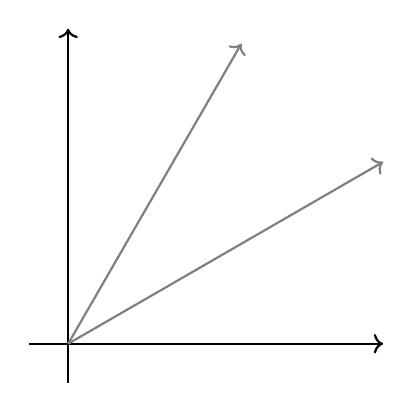
\begin{tikzpicture}
      		\draw[->,thick] (-0.5,0) -- (4,0);
      		\draw[->,thick] (0,-0.5) -- (0,4);
      		\draw[gray,thick,->,domain=0:4] plot (\x,{\x/sqrt(3)});
      		\draw[gray,thick,->,domain=0:2.2] plot (\x,{sqrt(3)*\x});
    	    \end{tikzpicture}         
          }  
          \caption*{$\sigma_1$}
          \label{fig:A}
     \end{subfigure}
     \begin{subfigure}[b]{0.325\textwidth}
          \centering
          \resizebox{0.8 \linewidth}{!}{
              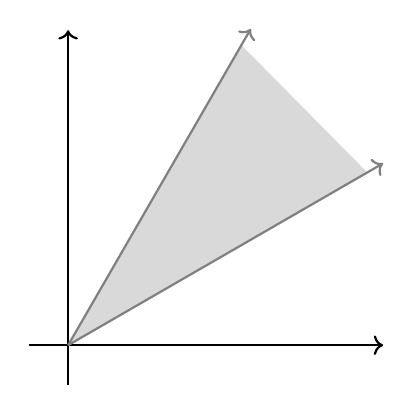
\begin{tikzpicture}
      		\draw[->,thick] (-0.5,0) -- (4,0);
      		\draw[->,thick] (0,-0.5) -- (0,4);
		    \fill[gray!30] (0,0) -- plot[domain=0:3.8] (\x,{\x/sqrt(3)}) -- plot[domain=2.2:0] (\x,{sqrt(3)*\x}) -- cycle;
      		\draw[gray,thick,->,domain=0:4] plot (\x,{\x/sqrt(3)});
      		\draw[gray,thick,->,domain=0:2.32] plot (\x,{sqrt(3)*\x});
    	\end{tikzpicture}          
          }  
          \caption*{$\sigma_2$}
          \label{fig:B}
     \end{subfigure}
     \begin{subfigure}[b]{0.325\textwidth}
          \centering
          \resizebox{\linewidth}{!}{
              \begin{tikzpicture}[tdplot_main_coords]
				\coordinate (O) at (0,0,1);
         		 \draw (0,0,-1) -- (O);
      			 \draw[->] (-5,0,1) -- (5,0,1) node[right] {};
     		 	 \draw[->] (0,-5,1) -- (0,5,1) node[right] {};
     		     \coneback[surface]{3}{2}{11}
     		     \draw[->] (O) -- (0,0,5) node[above] {};
      		     \conefront[surface]{3}{2}{13}
   	 \end{tikzpicture}
          }  
          \caption*{$\sigma_3$}
          \label{fig:C}
     \end{subfigure}
 \end{figure}
\end{example}

\begin{definition}
Let $\sigma$ be a cone.
The \emph{dual cone} $\sigma^\vee$ is
$$\sigma^\vee = \{u \in M_\RR : \langle u, v \rangle \ge 0 \text{ for all } v \in \sigma\}.$$
\end{definition}

\begin{example}
In the following examples, we let $N = \ZZ^n \subseteq \RR^n \cong N_\RR$, with standard basis $e_1, \ldots, e_n$.
Let $e_1^*, \ldots, e_n^*$ be the dual basis for $M$.
\begin{enumerate}
\item
Let $\sigma = \Span_{\RR_{\ge 0}}\{e_1, \ldots, e_n\},$ the \emph{positive orthant}.
Observe that a functional $\sum_{i=1}^n a_i e_i^*$ is in the dual cone if and only $a_i \ge 0$ for all $i$.
Then $\sigma^\vee = \Span_{\ge 0}\{e_1^*, \ldots, e_n^*\}$.

\item
Let $n = 2$ and let $\sigma = \Span_{\RR_{\ge 0}} \{e_1, - e_1 + 2 e_2\}.$
If $u \in M_\RR$, checking $\langle u, v \rangle \ge 0$ for all $v \in \sigma$ is equivalent to checking for the generators $v = e_1$ and $v = -e_1 + 2 e_2$.
So then $u = a e_1^* + b e_2^* \in M_\RR$ is in $\sigma^\vee$ exactly when the following two inequalities hold:
$$\langle u, e_1 \rangle = a \ge 0, \quad \langle u, -e_1 + 2e_2 \rangle = -a + 2b \ge 0.$$
Below we have a sketch of $\sigma$ and $\sigma^\vee$:
\begin{figure}[H]
    \centering
    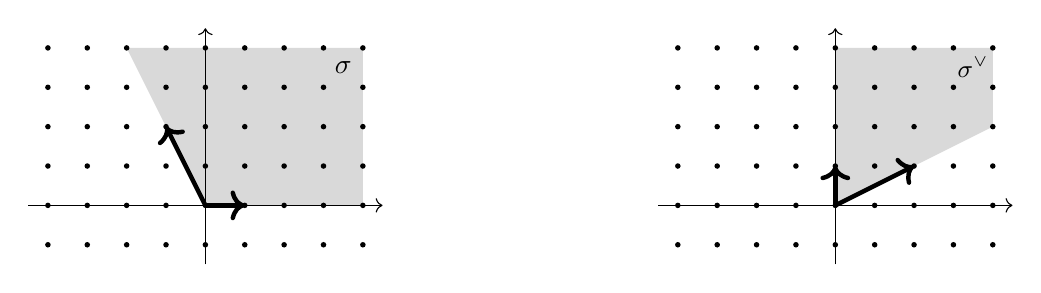
\begin{tikzpicture}
        % Left diagram
        \begin{scope}[shift={(-4,0)}]
            % Shaded area
            \fill[gray!30] (0,0) -- (-1,2) -- (2,2) -- (2,0) -- cycle;
            
            % Axes
            \draw[->] (-2.25,0) -- (2.25,0);
            \draw[->] (0,-0.75) -- (0,2.25);
            
            % Lattice points
            \foreach \x in {-2,-1.5,-1,-0.5,0,0.5,1,1.5,2}
                \foreach \y in {-0.5,0,0.5,1,1.5,2}
                    \fill (\x,\y) circle (1pt);

            % Vectors
            \draw[->, ultra thick] (0,0) -- (0.5,0);
            \draw[->, ultra thick] (0,0) -- (-0.5,1);
            \node at (1.75, 1.75) {$\sigma$};
        \end{scope}
        
        % Right diagram
        \begin{scope}[shift={(4,0)}]
            % Shaded area
            \fill[gray!30] (0,0) -- (0,2) -- (2,2) -- (2, 1) -- cycle;
            
            % Axes
            \draw[->] (-2.25,0) -- (2.25,0);
            \draw[->] (0,-0.75) -- (0,2.25);
            
            % Lattice points
            \foreach \x in {-2,-1.5,-1,-0.5,0,0.5,1,1.5,2}
                \foreach \y in {-0.5,0,0.5,1,1.5,2}
                    \fill (\x,\y) circle (1pt);

            % Vectors
            \draw[->, ultra thick] (0,0) -- (0,0.5);
            \draw[->, ultra thick] (0,0) -- (1,0.5);
            \node at (1.75, 1.75) {\small{$\sigma^\vee$}};
        \end{scope}
    \end{tikzpicture}
\end{figure}
\noindent
Then we can see that $\sigma^\vee = \Span_{\RR_{\ge 0}} \{2 e_1 + e_2, e_2\}.$
\end{enumerate}
\end{example}

The following theorem is a fundamental fact which relates a cone to its dual:

\begin{theorem}[{\cite[\S 1.2]{Fulton93}}]\label{dualitythm}
Let $\sigma$ be a closed convex cone in $N_\RR$.
If $v_0 \notin \sigma$, then there exists $u_0 \in \sigma^\vee$ such that $\langle u_0, v_0 \rangle <0.$
\end{theorem}

Despite its importance in the theory of toric varieties, most references on toric varieties such as \cite{Fulton93} and \cite{CLS11} do not prove it.
We give a proof here for completeness.
We begin with a lemma from analysis.

\begin{lemma}\label{mindistancelemma}
Let $A$ and $B$ be disjoint closed subsets of a finite-dimensional normed vector space $(V, \|\cdot\|)$, and assume $A$ is compact.
Then there exist $a_0 \in A$ and $b_0 \in B$ which minimise the distance $\|a-b\|$ over all $a \in A$ and $b \in B$.
\end{lemma}
%%%% THIS IS A WIKIPEDIA PROOF; FIND A REFERENCE %%%
\begin{proof}
Take arbitrary $a \in A$ and $b \in B$ and set $r_1 = \|a-b\| > 0$.
Since $A$ is compact, there exists $r_2 > 0$ such that $A \subseteq \overline{B_{r_2}(a)}$.
Let
$S = B \cap \overline{B_{r_1+r_2}(a)},$
which is nonempty since $b \in S$.
Since the distance function is continuous and $A \times S$ is compact, there exist $(a_0, b_0) \in A \times S$ minimising the distance $\|a_0 - b_0\|$ for all pairs of points in $A \times S$.
We claim that this is in fact the minimum for all pairs of points in $A \times B$; 
suppose to the contrary that there is $(a', b') \in A \times B$ with $\|a' - b'\| < \|a_0 - b_0\|$. 
In particular, since $\|a_0 - b_0\|\le r_1$, $\|a' - b'\| < r_1$ and so
$\|a - b'\| \le \|a - a'\| + \|a' - b'\| < r_2 + r_1.$
This implies $b' \in S$, contradicting that $\|a_0-b_0\|$ attained the minimum distance for pairs in $A \times S$.
\end{proof}

\begin{theorem}[Hyperplane Separation Theorem; {\cite[\S 2.5.1]{BV04}}]\label{hyperplaneseparation}
Let $A$ and $B$ be nonempty disjoint closed convex sets in a Euclidean vector space $(V, (\cdot,\cdot))$, and assume $A$ is compact.
Then there exists $v \in V$ and $\lambda \in \RR$ such that for all $a \in A$, $(v, a) \le \lambda$, and for all $b \in B$, $(v, b) \ge \lambda$.
In other words, there is an affine hyperplane such that $A$ is contained in the negative halfspace and $B$ is contained in the positive halfspace.
\end{theorem}

\begin{proof}
Lemma \ref{mindistancelemma} yields $a_0 \in A$ and $b_0 \in B$ minimising the distance between points in $A$ and points in $B$.
Define
$$v := b_0 - a_0, \qquad \lambda := \frac{\|b_0\|^2 - \|a_0\|^2}{2} = \frac{1}{2}(b_0 - a_0, b_0 + a_0).$$
The set of $x \in V$ satisfying $(v, x) = \lambda$ is the hyperplane orthogonal to the line segment joining $a_0$ and $b_0$, and passing through its midpoint.
Let us prove that $(v, b) \ge \lambda$ for all $b \in B$ (a similar argument shows $(v, a) \le \lambda$ for all $a \in A$).
Assume for a contradiction that there exists $u \in B$ with $(v, u) < \lambda$.
Then,
\begin{align*}
	(v, u) - \frac{1}{2}(v, b_0 + a_0) < 0
							 \implies (v, u - b_0 + \frac{1}{2} (b_0 - a_0)) < 0
							 \implies (v, u - b_0) + \frac{1}{2} \|v\|^2 < 0.
\end{align*}
Thus $(v, u - b_0) < 0$.
Using the Leibniz rule for differentiating inner products, we see
$$\left. \frac{d}{dt} \|v + t(u - b_0)\|^2 \right|_{t=0} = \left. 2 (v + t(u-b_0), u - b_0) \right|_{t=0} = 2 (v, u - b_0) < 0,$$
so for small $t > 0$, we have
$$\|v + t(u - b_0)\| = \|b_0 + t(u - b_0) - a_0\| < \|v\| = \|b_0 - a_0\|.$$
But $B$ is convex and $b_0, u \in B$, so $(b_0 + t (u - b_0)) \in B$ when $t$ is sufficiently small.
This contradicts the minimality of $\|b_0 - a_0\|$.
\end{proof}

\begin{proof}[Proof of Theorem \ref{dualitythm} \textup{(\cite[Example 2.20]{BV04})}]
Fix a basis $e_1, \ldots, e_n$ for $N_\RR$ and endow $N_\RR$ with the Euclidean inner product which makes the basis orthonormal (i.e., $(e_i, e_j) = \delta_{ij}$).
Since $\sigma$ is closed and $v_0 \notin \sigma$, there exists $\varepsilon > 0$ such that $\overline{B_\varepsilon(v_0)}$ does not intersect $\sigma$.
By Theorem \ref{hyperplaneseparation}, there exist $v \in N_\RR$ and $\lambda \in \RR$ such that 
$$(v, x) \ge \lambda \qquad \text{and} \qquad (v, y) \le \lambda$$
for all $x \in \sigma$ and all $y \in \overline{B_\varepsilon(v_0)}$.
Since $x = 0 \in \sigma$, $\lambda \le 0$.
In fact, we claim that $(v, x) \ge 0$ for all $x \in \sigma$ and $(v, v_0) < 0$;
this completes the proof as then $u_0 := (x \mapsto (v, x))$ is a linear form in $\sigma^\vee$ with $\langle u_0, v_0 \rangle < 0$.
Suppose there exists $x \in \sigma$ with $(v, x) = \lambda_0 < 0$.
Then for any $s \in \RR_{\ge 0}$, $s x \in \sigma $ and $(v, s x) = s \lambda_0$, contradicting that $\{(v, x) : x \in \sigma\}$ is bounded from below.
Assume for a contradiction $(v, v_0) = 0$.
We have $y = v_0 + \frac{\varepsilon v}{\|v\|} \in \overline{B_\varepsilon(v_0)}$ and
$$0 \ge \lambda \ge (v, y) = (v, v_0 + \frac{\varepsilon v}{\|v\|}) = \varepsilon \|v\| > 0,$$
a contradiction.
\end{proof}

\begin{corollary}
Let $\sigma$ be a closed cone in $N_\RR$.
Then $(\sigma^\vee)^\vee = \sigma$.
\end{corollary}
\begin{proof}
If $v \in \sigma$, $\langle u, v\rangle \ge 0$ for all $u \in \sigma^\vee$, so $v \in (\sigma^\vee)^\vee$.
If $v \notin \sigma$, Theorem \ref{dualitythm} implies there exists $u \in \sigma^\vee$ with $\langle u, v \rangle < 0$ and hence $v \notin (\sigma^\vee)^\vee$.
\end{proof}

\subsection{Polyhedral cones} 
In the study of toric varieties, we are interested in the following class of closed convex cones:

\begin{definition}\label{convexpolyhedraldef}
A subset $\sigma \subseteq N_\RR$ is a \emph{convex polyhedral cone} if
$$\sigma = \Span_{\RR_{\ge 0}} \{v_1, \ldots, v_s\}$$
for a (finite) set of generators $v_1, \ldots, v_s \in N_\RR$.
\end{definition}

It follows from the definition that convex polyhedral cones are indeed convex cones.
Every example of a cone we have seen so far has been polyhedral, except for $\sigma_3 = \{(x, r) \in \RR^2 \times \RR : \|x\| \le r\}$ in Example \ref{coneexamples}.
As given, a more apt name for this definition would be ``finitely-generated cone'';
the name polyhedral is justified by the fact that a cone satisfies Definition \ref{convexpolyhedraldef} if and only if it is a finite intersection of closed halfspaces with $0$ on their boundary (i.e., is polyhedral)---see \cite[\S 1.3]{DLHK13} for a proof.

Fulton \cite[\S 1.2]{Fulton93} states and proves many important consequences of Theorem \ref{dualitythm} for convex polyhedral cones.
We explain a few of these now.

Any $u \in M_\RR$ defines a hyperplane, denoted $u^\perp$, and corresponding nonnegative halfspace $u^\vee$.
These are defined as
$$u^\perp := \{v \in N_\RR : \langle u, v\rangle = 0\}, \qquad u^\vee := \{v \in N_\RR : \langle u, v\rangle \ge 0\}.$$
A face $\tau$ of $\sigma$ is the intersection of $\sigma$ with a hyperplane which is nonnegative on $\sigma$:
$$\tau = \sigma \cap u^\perp = \{v \in \sigma : \langle u, v \rangle = 0\}, \qquad \text{for some } u \in \sigma^\vee.$$
A facet is a codimension one face. 
Any proper face is the intersection of all facets containing it.
When $\sigma$ spans $N_\RR$ and $\tau$ is a facet of $\sigma$, there exists $u \in \sigma^\vee$, which is unique up to multiplication by a positive scalar, such that
$$\tau = \sigma \cap u^\perp.$$
We denote such a vector by $u_\tau$, which gives the equation for the hyperplane spanned by $\tau$.
The face $\sigma \cap u^\perp$ is generated by the vectors $v_i$ in the generating set for $\sigma$ such that $\langle u, v_i\rangle = 0$.
If $\sigma$ spans $N_\RR$, the dual cone is generated by $\{u_\tau : \tau \text{ is a facet }\}$.
This implies the dual of a convex polyhedral cone is also a convex polyhedral cone (this result is true without assuming $\sigma$ spans $N_\RR$).
Example \ref{coneanddualexample} below gives an example of computing facets and dual cone generators.

\begin{example}\label{coneanddualexample}
Let $N = \ZZ^3$ and let $\sigma = \Span_{\RR_{\ge 0}}\{ e_1, e_2, e_1+e_3, e_2 + e_3\} \subseteq N_\RR \cong \RR^3$.
Observe that 
$$u_{\tau_1} = e_1^*, \,\,\,\,\,\,\,\,\,\, u_{\tau_2} = e_2^*, \,\,\,\,\,\,\,\,\,\, u_{\tau_3} = e_3^*, \,\,\,\,\,\,\,\,\,\, u_{\tau_4} = e_1^* + e_2^* - e_3^*$$
are all nonnegative on $\sigma$ and hence lie in $\sigma^\vee$. 
For each $u_{\tau_i}$, there is the corresponding facet $\tau_i = \sigma \cap u_{\tau_i}^\perp$.

These are:
\begin{align*}
	&\tau_1 = \Span_{\RR_{\ge 0}}\{e_2, e_2+e_3\}, & &\tau_2 = \Span_{\RR_{\ge 0}} \{e_1, e_1+e_3\}, \\
	&\tau_3 = \Span_{\RR_{\ge 0}}\{e_1, e_2\},  & &\tau_4 = \Span_{\RR_{\ge 0}} \{e_1+e_3, e_2+e_3\}.
\end{align*}
The other faces in $\sigma$ are the rays 
\begin{align*}
	&\tau_1 \cap \tau_3 = \Span_{\RR_{\ge 0}}\{e_2\}, & &\tau_1 \cap \tau_4 = \Span_{\RR_{\ge 0}} \{e_2+e_3\}, \\
	&\tau_2 \cap \tau_3 = \Span_{\RR_{\ge 0}}\{e_1\}, & &\tau_2 \cap \tau_4 = \Span_{\RR_{\ge 0}} \{e_1+e_3\},
\end{align*}
and the origin $\bigcap_{i=1}^4 \tau_i = \{0\}.$
The dual cone is
$$\sigma^\vee = \Span_{\RR_{\ge 0}} \{e_1^*, e_2^*, e_3^*, e_1^* +e_2^* - e_3^*\}.$$

\begin{figure}[H]
\includegraphics[width=0.2 \textwidth]{../images/cox cone example 2}
\caption*{A diagram of $\sigma$ \cite[Figure 2]{CLS11}}
\end{figure}

\end{example}

\subsection{The semigroup of a cone}
Recall that a monoid is a group where elements do not necessarily have inverses;
specifically, a monoid is a set with an associative binary operation with identity.
In the study of toric varieties, we construct a monoid $S_\sigma$ from a cone $\sigma$.
In toric varieties literature, it is typical to refer to $S_\sigma$ as a \emph{semigroup} (a set with an assoicative binary operation) even though calling it a monoid would be more precise.
We follow the convention of calling $S_\sigma$ a semigroup; let us now describe the construction.

A convex polyhedral cone $\sigma \subseteq N_\RR$ is called \emph{rational} it can be generated by elements in the lattice $N$.
When $\sigma$ is rational, $\sigma^\vee$ is also rational.
Given a rational convex polyhedral cone $\sigma$, the semigroup of $\sigma$ is
$$S_\sigma = \sigma^\vee \cap M.$$

\begin{theorem}[Gordan's lemma, {\cite[\S 1.2]{Fulton93}}]\label{gordanslemma}
If $\sigma$ is a rational convex polyhedral cone, then $S_\sigma = \sigma^\vee \cap M$ is a finitely generated semigroup.
\end{theorem}
\begin{proof}
Let $u_1, \ldots, u_s \in \sigma^\vee \cap M$ generate $\sigma^\vee$ as a cone.
Define
$$K = \left\{\sum t_i u_i : 0 \le t_i \le 1\right\}.$$
Since $K$ is compact and $M$ is discrete, the intersection $K \cap M$ is finite, and we claim is a generating set for $S_\sigma$.
Note that $u_1, \ldots, u_s \in K \cap M$.
Suppose that $u \in S_\sigma$.
Then $u = \sum r_i u_i$ for some $r_i \in \RR_{\ge 0}$ since the $u_i$ generate $\sigma^\vee$.
Write each $r_i$ as $m_i + t_i$ for $m_i \in \ZZ_{\ge 0}$ and $0 \le t_i \le 1$, so $u = \sum m_i u_i + \sum t_i u_i$.
Clearly $\sum t_i u_t \in K$.
Also, $\sum t_i u_t = u - \sum m_i u_i \in M$ since $u, \sum m_i u_i \in M$ and $M$ is a group.
Then $\sum t_i u_t \in K \cap M$, and $u = \sum m_i u_i + \sum t_i u_i$ shows $u \in \Span_{\ZZ_{\ge 0}} K \cap M$.
\end{proof}

\begin{proposition}[{\cite[\S 1.2, Proposition 3]{Fulton93}}]\label{stronglyconvexprop}
For a convex polyhedral cone $\sigma$, the following conditions are equivalent:
\begin{enumerate}
\item $\sigma \cap (-\sigma) = \{0\}$;
\item $\sigma$ contains no nonzero linear subspace;
\item there is $u \in \sigma^\vee$ with $\sigma \cap u^\perp = \{0\}$;
\item $\sigma^\vee$ spans $M_\RR$.
\end{enumerate}
\end{proposition}

A cone is called \emph{strongly convex} if it satisfies the conditions of Proposition \ref{stronglyconvexprop}.
In the study of toric varieties, one works with strongly convex cones.
This ensures the dual cone $\sigma^\vee$ spans $M_\RR$ so that the semigroup $S_\sigma = \sigma^\vee \cap M$ is not ``too small''.
In particular, we will see later that the strongly convex assumption is needed to prove that the toric variety defined by a cone indeed has a torus as a dense open subset.

Moving forward, we will say ``$\sigma$ is a cone in $N$'' to mean $\sigma$ is a strongly convex rational polyhedral cone in $N_\RR$.

\subsection{The semigroup algebra and affine toric varieties}
Given a cone $\sigma$, we have seen how to construct a semigroup $S_\sigma = \sigma^\vee \cap M$.
There is a corresponding semigroup algebra $\CC[S_\sigma]$, which is a finitely generated commutative $\CC$-algebra.

\begin{definition}
Let $\sigma$ be a rational cone in $N$.
We define the affine toric variety corresponding to $\sigma$ to be
$$U_\sigma := \Spec(\CC[S_\sigma]).$$
\end{definition}

Let us explain the details of the construction.
Given the semigroup $S_\sigma = \sigma^\vee \cap M$, the semigroup algebra $\CC[S_\sigma]$ is defined as having a basis of formal symbols
$$\{\chi^u : u \in S_\sigma\},$$
with multiplication determined by addition in $S_\sigma$:
$$\chi^u \cdot \chi^{u'} = \chi^{u + u'}.$$
Note the multiplication is commutative since $S_\sigma$ is.
We have the unit $\chi^0 \in \CC[S_\sigma]$ corresponding to the unit $0 \in S_\sigma$.
By Theorem \ref{gordanslemma}, $S_\sigma$ has a finite generating set $\{u_i\}$.
Then $\{\chi^{u_i}\}$ generate $\CC[S_\sigma]$, and $\CC[S_\sigma]$ is a finitely generated $\CC$-algebra.

We can think of $\CC[S_\sigma]$ as a subalgebra of the ring of Laurent polynomials in the following way:
when $\sigma = \{0\}$, the dual cone is all of $M_\RR$, so $S_{\{0\}} = M$;
if $e_1, \ldots, e_n$ is a basis for $N$ and $e_1^*, \ldots, e_n^*$ is the dual basis, denote
$$X_i = \chi^{e_i^*} \in \CC[M].$$
As a semigroup, $M$ is generated by $\pm e_1^*, \ldots, \pm e_n^*$, so
$$\CC[S_{\{0\}}] = \CC[M] = \CC[X_1^\pm, \ldots, X_n^\pm].$$
For any cone $\sigma$, $\{0\} \subseteq \sigma$, which implies $\{0\}^\vee \supseteq \sigma^\vee$ and $S_{\{0\}} = \{0\}^\vee \cap M \supseteq S_\sigma = \sigma^\vee \cap M.$
Then we can think of $\CC[S_\sigma]$ as a subalgebra of the Laurent polynomials.

As $\CC[S_\sigma]$ is a finitely generated $\CC$-algebra, $U_\sigma = \Spec(\CC[S_\sigma])$ is a complex affine variety.
For example, when $\sigma = \{0\}$ so that $\CC[S_\sigma] = \CC[X_1^\pm, \ldots, X_n^\pm]$, 
$$U_{\{0\}} = \mathrm{Specm}(\CC[X_1^\pm, \ldots, X_n^\pm]) = (\CC^\times)^n.$$

\begin{example}
Let us see more examples arising from the cones we have seen previously.
\begin{enumerate}
\item
For $\sigma = \Span_{\RR_{\ge 0}}\{e_1, \ldots, e_n\},$ 
$$\sigma^\vee = \Span_{\RR_{\ge 0}}\{e_1^*, \ldots, e_n^*\}.$$
Then vectors $e_1^*, \ldots, e_n^*$ generate $S_\sigma$ as a semigroup, so
$$\CC[S_\sigma] = \CC[\chi^{e_1^*}, \ldots, \chi^{e_n^*}] = \CC[X_1, \ldots, X_n],$$
and 
$$U_\sigma = \mathrm{Specm}(\CC[X_1, \ldots, X_n]) = \CC^n.$$

\item
Recall that for $\sigma = \Span_{\RR_{\ge 0}} \{e_1, - e_1 + 2 e_2\}$,
$$\sigma^\vee = \Span_{\RR_{\ge 0}} \{2 e_1^* + e_2^*, e_2^*\}.$$
\begin{figure}[H]
    \centering
    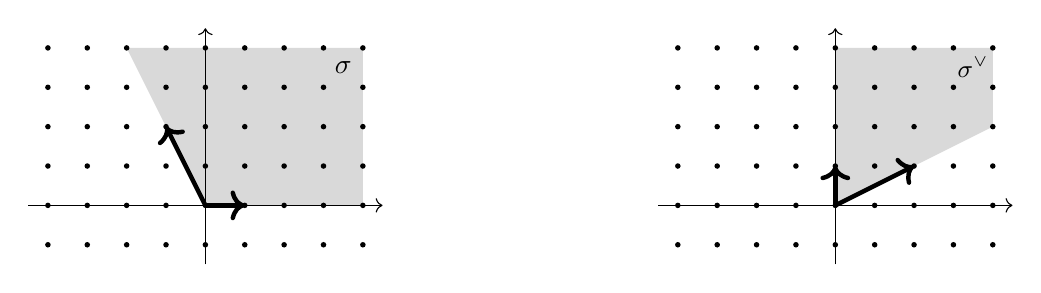
\begin{tikzpicture}
        % Left diagram
        \begin{scope}[shift={(-4,0)}]
            % Shaded area
            \fill[gray!30] (0,0) -- (-1,2) -- (2,2) -- (2,0) -- cycle;
            
            % Axes
            \draw[->] (-2.25,0) -- (2.25,0);
            \draw[->] (0,-0.75) -- (0,2.25);
            
            % Lattice points
            \foreach \x in {-2,-1.5,-1,-0.5,0,0.5,1,1.5,2}
                \foreach \y in {-0.5,0,0.5,1,1.5,2}
                    \fill (\x,\y) circle (1pt);

            % Vectors
            \draw[->, ultra thick] (0,0) -- (0.5,0);
            \draw[->, ultra thick] (0,0) -- (-0.5,1);
            \node at (1.75, 1.75) {$\sigma$};
        \end{scope}
        
        % Right diagram
        \begin{scope}[shift={(4,0)}]
            % Shaded area
            \fill[gray!30] (0,0) -- (0,2) -- (2,2) -- (2, 1) -- cycle;
            
            % Axes
            \draw[->] (-2.25,0) -- (2.25,0);
            \draw[->] (0,-0.75) -- (0,2.25);
            
            % Lattice points
            \foreach \x in {-2,-1.5,-1,-0.5,0,0.5,1,1.5,2}
                \foreach \y in {-0.5,0,0.5,1,1.5,2}
                    \fill (\x,\y) circle (1pt);

            % Vectors
            \draw[->, ultra thick] (0,0) -- (0,0.5);
            \draw[->, ultra thick] (0,0) -- (1,0.5);
            \node at (1.75, 1.75) {\small{$\sigma^\vee$}};
        \end{scope}
    \end{tikzpicture}
\end{figure}
\noindent
Observe that while $2 e_1^* + e_2^*$ and $e_2^*$ generate $\sigma^\vee$ as a cone, they do not generate $S_\sigma$ as a semigroup.
For example, $e_1^* + e_2^* \in S_\sigma$ but $e_1^* + e_2^* \notin \ZZ_{\ge 0} \cdot (2 e_1^* + e_2^*) + \ZZ_{\ge 0} \cdot e_2^*.$
However, $e_2^*, e_1^* + e_2^*, 2 e_1^* + e_2^*$ do generate $S_\sigma$.
Then
\begin{align*}
	\qquad \CC[S_\sigma] = \CC[\chi^{e_2^*}, \chi^{e_1^* + e_2^*}, \chi^{2 e_1^* + e_2^*}] &= \CC[X_2, X_1 X_2, X_1^2 X_2] = \CC[U, V, W] / (U W - V^2)
\end{align*}

\item
For $\sigma = \Span_{\RR_{\ge 0}}\{ e_1, e_2, e_1+e_3, e_2 + e_3\}$, we saw
$$\sigma^\vee = \Span_{\RR_{\ge 0}} \{e_1^*, e_2^*, e_3^*, e_1^* +e_2^* - e_3^*\}.$$
Then 
\begin{align*}
	\CC[S_\sigma] = \CC[\chi^{e_1^*}, \chi^{e_2^*}, \chi^{e_3^*}, \chi^{e_1^* +e_2^* - e_3^*}] &= \CC[X_1, X_2, X_3, X_1 X_2 X_3^{-1}] \\
	&= \CC[X, Y, Z, W]/(XY - ZW)
\end{align*}

\end{enumerate}
\end{example}

\subsection{$\AA^n \git T$ as a toric variety}
In this section, we will study how the GIT quotient of a torus acting on affine space can be given the structure of a toric variety.
We follow \cite[\S 12]{Dolgachev03}.

Let $T = \mathbb{G}_m^r$ act linearly on $\AA^n$ by
$$t \cdot (z_1, \ldots, z_n) = (t^{\mathbf{a}_1} z_1, \ldots, t^{\mathbf{a}_n} z_n),$$
where if $t = (t_1, \ldots, t_r)$ and $\mathbf{a}_j = (a_{1j}, \ldots, a_{rj}) \in \ZZ^r$,
$$t^{\mathbf{a}_j} = t_1^{a_{1j}} \cdots t^{a_{rj}}.$$
Note that any representation of $T$ can be written this way, after diagonalising the action.
A polynomial $F \in k[Z_1, \ldots, Z_n]$ is invariant if and only if it is a linear combination of monomials $Z^\mathbf{m}$ satisfying
\begin{equation}\label{invsys}
	A \cdot \mathbf{m} = 0.
\end{equation}
% \todo{More explanation required, though this is shown properly when we look at $\CC[\frakg]^T$.}
Here $A = (a_{ij})$ is the $n \times r$ matrix of the exponents of the characters that $T$ acts by.
Let $\mathcal{M}$ be the semigroup of vectors $\mathbf{m} \in \ZZ_{\ge 0}^n$ satisfying equation \ref{invsys}.
Since these $\mathbf{m}$ are precisely the exponents of invariant monomials for the action of $T$ on $\AA^n$, we have the isomorphism
$$k[Z_1, \ldots, Z_n]^T = k[Z^\mathbf{m} : A \cdot \mathbf{m} = 0] \cong k[\mathcal{M}].$$

To give $\AA^n \git T$ the structure of a toric variety, we need to find a lattice $N$ and a cone $\sigma$ in $N_\RR$ such that $\mathcal{M} \cong \sigma^\vee \cap M$.
To this end, let $\ZZ^n \to \ZZ^r$ be the map given by the matrix $A$, and let $M = N^*$ be be the kernel of this map.
Then $M$ is a free abelian group of rank $l = n - \mathrm{rank}(A)$.
Let $(\ZZ^n)^* \to N = M^*$ be the map given by restriction of linear functions to $M$.
Let $e_1^*, \ldots, e_n^*$ be the dual basis of the standard basis $e_1, \ldots, e_n$ for $\ZZ^n$, and let $\bar{e}_1^*, \ldots, \bar{e}_n^*$ be the image of these vectors in $M^*$.
We define $\sigma$ to be the convex cone in $N_\RR$ generated by the vectors $\bar{e}_1^*, \ldots, \bar{e}_n^*$, i.e.,
$$\sigma = \RR_{\ge 0} \cdot \bar{e}_1^* + \ldots +\RR_{\ge 0} \cdot \bar{e}_n^*.$$

\begin{lemma}
We have that $\sigma^\vee \cap M = \mathcal{M}$, such that
$$k[Z_1, \ldots, Z_n]^T \cong k[\mathcal{M}] = k[\sigma^\vee \cap M].$$
Thus $\AA^n \git T$ is isomorphic to the affine toric variety defined by the cone $\sigma$.
\end{lemma}
\begin{proof}
Note that $\mathcal{M} = M \cap \mathbb{Z}_{\ge 0}^n$.
Then
\begin{align*}
	\mathcal{M} &= \{m \in M : \bar{e}_i^*(m) \ge 0 \text{ for all } i = 1, \ldots, n\} \\
			&= \{m \in M : n(m) \ge 0 \text{ for all } n \in \sigma\} \\
			&= \sigma^\vee \cap M.
\end{align*}
\end{proof}

\subsection{Properties of toric varieties}
%\textcolor{red}{
%This section is an attempt to indicate why we might be interested in using the toric variety structure to study $\AA^n \git T$ and specifically $\frakg \git T$,
%but these are things I'm still trying to understand.
%}
%Suppose we have a cone $\sigma$ and the corresponding affine toric variety $U_\sigma$.
%For any face $\tau$ of the cone $\sigma$, we have the inclusion $\tau \hookrightarrow \sigma$, implying $\tau^\vee \hookleftarrow \sigma^\vee$, 
%$S_\tau = \tau^\vee \cap M \hookleftarrow  \sigma^\vee \cap M = S_\sigma$ and
%$$\CC[S_\tau] \hookleftarrow \CC[S_\sigma].$$
%Correspondingly there is a morphism
%$$U_\tau = \mathrm{Specm}(\CC[S_\tau]) \to U_\sigma = \mathrm{Specm}(\CC[S_\sigma]).$$
%In particular, this map embeds $U_\tau$ as a principal open subset of $U_\sigma$ (see \cite[\S 1.3]{Fulton93}).
%When $\tau = \{0\}$, $U_{\{0\}} = (\CC^\times)^n$, where $n$ is the dimension of $N$.
%This is why toric varieties (defined in terms of cones) have a torus as a dense open subset.
%Also, the action of $U_{\{0\}} = (\CC^\times)^n =: T_N $ on itself extends to an action of $T_N$ on $U_\sigma$.
%The orbits of this action are in bijection with the faces of the cone $\sigma$.
%
%The cone $\sigma$ also contains information about the singularities of $U_\sigma$.
%Specifically, $U_\sigma$ is nonsingular if and only if $\sigma$ is generated by a subset of a basis for $N$ (see \cite[\S 2.1]{Fulton93}).
%
%Combining these ideas about orbits of the torus action and singularities, the upshot is that we should be able to understand singular points by looking at the cone $\sigma$.
%
%\begin{example}
%Let 
%$$\sigma = \Span_{\RR_{\ge 0}} \{e_1, e_2, e_3, e_1 + e_4, e_2 + e_4, e_3 + e_4 \}.$$
%It can be computed (using the process described in \cite[page 11]{Fulton93}, or on a computer using Sage) that 
%$$\sigma^\vee = \Span_{\RR_{\ge 0}} \{e_1^*, e_2^*, e_3^*, e_1^* + e_2^* + e_3^* - e_4^* \}.$$
%It follows that the coordinate ring of $U_\sigma$ is
%$$\CC[S_\sigma] = \CC[X_1, X_2, X_3, X_4, X_1 X_2 X_3 X_4^{-1}] \cong \CC[X, Y, Z, U, V]/(XYZ - UV).$$
%\end{example}
%Then $U_\sigma$ is the variety $\bV(XYZ - UV) \subseteq \CC^5$, which is $\frakg \git T$ when $G = \GL_3$.
%If $\sigma^\vee \cap M$ is a generated by $\{a_1, \ldots, a_r\} \subseteq M \cong \ZZ^n$, 
%the action of the torus $T_N \cong (\CC^\times)^n$ on the variety can be given explicitly as 
%$$t \cdot (x_1, \ldots, x_r) = (t^{a_1} x_1, \ldots, t^{a_r} x_r).$$
%In this example, $T = (\CC^\times)^4$ acts on $\bV(XYZ - UV) \subseteq \CC^5$ by
%$$(t_1, t_2, t_3, t_4) \cdot (X, Y, Z, U, V) = (t_1 X, t_2 Y, t_3 Z, t_4 U, t_1 t_2 t_3 t_4^{-1} V).$$
%Using Sage, I computed that the facets (codimension one faces) are the following:
%\begin{align*}
%	\tau_1 &= \Span_{\RR_{\ge 0}} \{e_1, e_2, e_1 + e_4, e_2 + e_4\} \\
%	\tau_2 &= \Span_{\RR_{\ge 0}} \{e_2, e_3, e_2 + e_4, e_3 + e_4\} \\
%	\tau_3 &= \Span_{\RR_{\ge 0}} \{e_1, e_3, e_1 + e_4, e_3 + e_4\} \\
%	\tau_4 &= \Span_{\RR_{\ge 0}} \{e_1, e_2, e_3\} \\
%	\tau_5 &= \Span_{\RR_{\ge 0}} \{e_1 + e_4, e_2 + e_4, e_3 + e_4\} 
%\end{align*}
%Notice that $\tau_1, \tau_2$ and $\tau_3$ are not generated by subsets of a basis of $N$ while the other facets are.
%We also consider the cone $\sigma$ as a face of itself, which is also not generated by a subset of a basis for $N$.
%We then have the following correspondence:
%\begin{align*}
%	&\sigma & &\leftrightarrow &  &T_N \cdot (0, 0, 0, 0, 0) = (0, 0, 0, 0, 0) \\
%	&\tau_1 & &\leftrightarrow &  &T_N \cdot (1, 0, 0, 0, 0) =  \CC^\times \times \{0\}^4 \\
%	&\tau_2 & &\leftrightarrow &  &T_N \cdot (0, 1, 0, 0, 0) = \{0\} \times \CC^\times \times \{0\}^3 \\
%	&\tau_3 & &\leftrightarrow &  &T_N \cdot (0, 0, 1, 0, 0) =  \{0\}^2 \times \CC^\times \times \{0\}^2 
%\end{align*}
%The union of these three orbits is precisely the singular locus of $U_\sigma$.






%%%%%%%%%%%%%%%%%%%%%%%%%%%%%%%%%%%%%%%%%%%%%%%%%%%%%%%%%%%%%%%%%%%%%%%%%%%%%%%%
% REFERENCES
%%%%%%%%%%%%%%%%%%%%%%%%%%%%%%%%%%%%%%%%%%%%%%%%%%%%%%%%%%%%%%%%%%%%%%%%%%%%%%%%
\newpage
\begin{bibdiv}
\begin{biblist}
\bib{BV04}{book}{
   author={Boyd, Stephen},
   author={Vandenberghe, Lieven},
   title={Convex optimization},
   publisher={Cambridge University Press, Cambridge},
   date={2004},
   pages={xiv+716},
   isbn={0-521-83378-7},
   review={\MR{2061575}},
   doi={10.1017/CBO9780511804441},
}

\bib{CLS11}{book}{
   author={Cox, David A.},
   author={Little, John B.},
   author={Schenck, Henry K.},
   title={Toric varieties},
   series={Graduate Studies in Mathematics},
   volume={124},
   publisher={American Mathematical Society, Providence, RI},
   date={2011},
   pages={xxiv+841},
   isbn={978-0-8218-4819-7},
   review={\MR{2810322}},
   doi={10.1090/gsm/124},
}

\bib{DLHK13}{book}{
   author={De Loera, Jes\'us A.},
   author={Hemmecke, Raymond},
   author={K\"oppe, Matthias},
   title={Algebraic and geometric ideas in the theory of discrete
   optimization},
   series={MOS-SIAM Series on Optimization},
   volume={14},
   publisher={Society for Industrial and Applied Mathematics (SIAM),
   Philadelphia, PA; Mathematical Optimization Society, Philadelphia, PA},
   date={2013},
   pages={xx+322},
   isbn={978-1-611972-43-6},
   review={\MR{3024570}},
}

\bib{Dolgachev03}{book}{
   author={Dolgachev, Igor},
   title={Lectures on invariant theory},
   series={London Mathematical Society Lecture Note Series},
   volume={296},
   publisher={Cambridge University Press, Cambridge},
   date={2003},
   pages={xvi+220},
   isbn={0-521-52548-9},
   review={\MR{2004511}},
   doi={10.1017/CBO9780511615436},
}

\bib{Fulton93}{book}{
   author={Fulton, William},
   title={Introduction to toric varieties},
   series={Annals of Mathematics Studies},
   volume={131},
   note={The William H. Roever Lectures in Geometry},
   publisher={Princeton University Press, Princeton, NJ},
   date={1993},
   pages={xii+157},
   isbn={0-691-00049-2},
   review={\MR{1234037}},
   doi={10.1515/9781400882526},
}

\bib{Hartshorne77}{book}{
   author={Hartshorne, Robin},
   title={Algebraic geometry},
   series={Graduate Texts in Mathematics},
   volume={No. 52},
   publisher={Springer-Verlag, New York-Heidelberg},
   date={1977},
   pages={xvi+496},
   isbn={0-387-90244-9},
   review={\MR{0463157}},
}

\bib{Humphreys72}{book}{
   author={Humphreys, James E.},
   title={Introduction to Lie algebras and representation theory},
   series={Graduate Texts in Mathematics},
   volume={Vol. 9},
   publisher={Springer-Verlag, New York-Berlin},
   date={1972},
   pages={xii+169},
   review={\MR{0323842}},
}

\bib{Reid88}{book}{
   author={Reid, Miles},
   title={Undergraduate algebraic geometry},
   series={London Mathematical Society Student Texts},
   volume={12},
   publisher={Cambridge University Press, Cambridge},
   date={1988},
   pages={viii+129},
   isbn={0-521-35559-1},
   isbn={0-521-35662-8},
   review={\MR{0982494}},
   doi={10.1017/CBO9781139163699},
}

\bib{Reid95}{book}{
   author={Reid, Miles},
   title={Undergraduate commutative algebra},
   series={London Mathematical Society Student Texts},
   volume={29},
   publisher={Cambridge University Press, Cambridge},
   date={1995},
   pages={xiv+153},
   isbn={0-521-45255-4},
   review={\MR{1458066}},
   doi={10.1017/CBO9781139172721},
}
\end{biblist}
\end{bibdiv}
\end{document}
